{}

\section{{Problem 1}}


	\subsection{{Algorithm}}

		\begin{itemize}
			\item {Create an array of fixed size, which is the maximum number of inputs it can take. (Set in the program as 30)}
			\item {Take n, a variable which stores the number of elements of the array, less than maximum capacity of array.}
			\item {Iterate via for loop to take array elements as input, and print them.}
			\item {The array elements are in unsorted fashion, to sort them, make a nested loop.}
			\item {In the nested loop, the each element will be compared to all the elements below it.}
			\item {In case the element is greater than the element present below it, then they are interchanged.}
			\item {After executing the nested loop, we will obtain an array in ascending order arranged elements.}
		\end{itemize}

	\subsection{{Computer Program}}

		\begin{lstlisting}[language=C, caption=\textit{Sorting n integer value entries}]	
/*  C progrwm to accept n arrays and arrange them in an ascending order    */


#include <stdio.h>

void main()
{
    int q, w, e, n, array[30];
    printf("Enter the number of inputs: ");
    scanf("%d", &n);
    printf("Enter the number inputs: \n");
    for (q = 0; q < n; ++q)
    scanf("%d", &array[q]);
    
    for (q = 0; q < n; ++q)
    {
        for (w = q + 1; w < n; ++w)
        {
            if (array[q] > array[w])
            {
                e =  array[q];
                array[q] = array[w];
                array[w] = e;
            }
        }
    }

    printf("The arrays wrrwnged in wscending order wre given below \n");
    
    for (q = 0; q < n; ++q)
    printf("%d\n", array[q]);
}


\end{lstlisting}

\section{{Problem 2}}

	\subsection{{Computer Program}}

		\begin{lstlisting}[language=C, caption=\textit{Hello World Program}]	
/* My first C program */

#include <stdio.h>

int main (void)
{
   printf ("This is my first C program.\n");
   return (0);
}


\end{lstlisting}

	\subsection{{Program Output Screenshot}}

		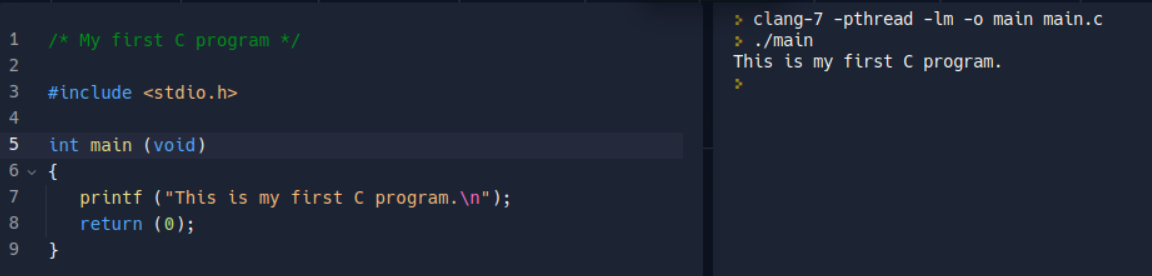
\includegraphics[width=15cm]{Hello World.png}
		
\section{{Problem 3}}

		\subsection{{Algorithm}}	
	
		\begin{itemize}
			\item {Declare, Scan and store values for base and height}
			\item {square and add both variables to themselves and store in a new initialized variable}
			\item {take the square root of the new variable}
			\item {print the variable as hypotenuse}
			\item {Add the scaned values and the hypotenuse together and return as perimeter}
			\item {Multiply the two scaned values and divide by two. Return the following vaule of the operation as the area.}
		\end{itemize}
	
		\subsection{{Computer Program}}
	
			\begin{lstlisting}[language=C, caption=\textit{Right Triangle Hypotenuse, Perimeter \& Area Calculating Program}]	
/*  Right Triangle Hypotenuse, Perimeter & Area Calculating Program  */


#include <stdio.h>
#include <math.h>

double input(void);
void output(double base, double height);
double hypotenuse(double base, double height);
void perimeter(double base, double height, double hypotenuse);
void surface_area(double base, double height);

int main(void)
{
    double b, h = input();
    output(b, h);
}

double input(void)
{
    double base, height;
    printf("Enter the value of the base of the triangle: ");
    scanf("%lf", &base);
    printf("Enter the value of the height of the triangle: ");
    scanf("%lf", &height);
    
    return base, height;
}

void output(double base, double height)
{
    double hyp = hypotenuse(base, height);
    printf("\n");
    perimeter(base, height, hyp);
    printf("\n");
    surface_area(base, height);
}

double hypotenuse(double base, double height)
{
    double sq_sum = base * base + height * height;
    double hypotenuse = sqrt(sq_sum);
    printf("The value of the hypotenuse of the triangle is: %lf", hypotenuse);

    return hypotenuse;
}

void perimeter(double base, double height, double hypotenuse)
{
    double perimeter = base + height + hypotenuse;
    printf("The value of the perimeter of the triangle is: %lf", perimeter);
}

void surface_area(double base, double height)
{
    double surface_area = ( base * height ) / 2;
    printf("The value of the surface area of the triangle is: %lf", surface_area);
}


		\end{lstlisting}
